\begin{frame}{Experimental Setup}{Materials}
%\begin{tabular}{ccc}
%	\begin{figure} 
%		\begin{center}
%			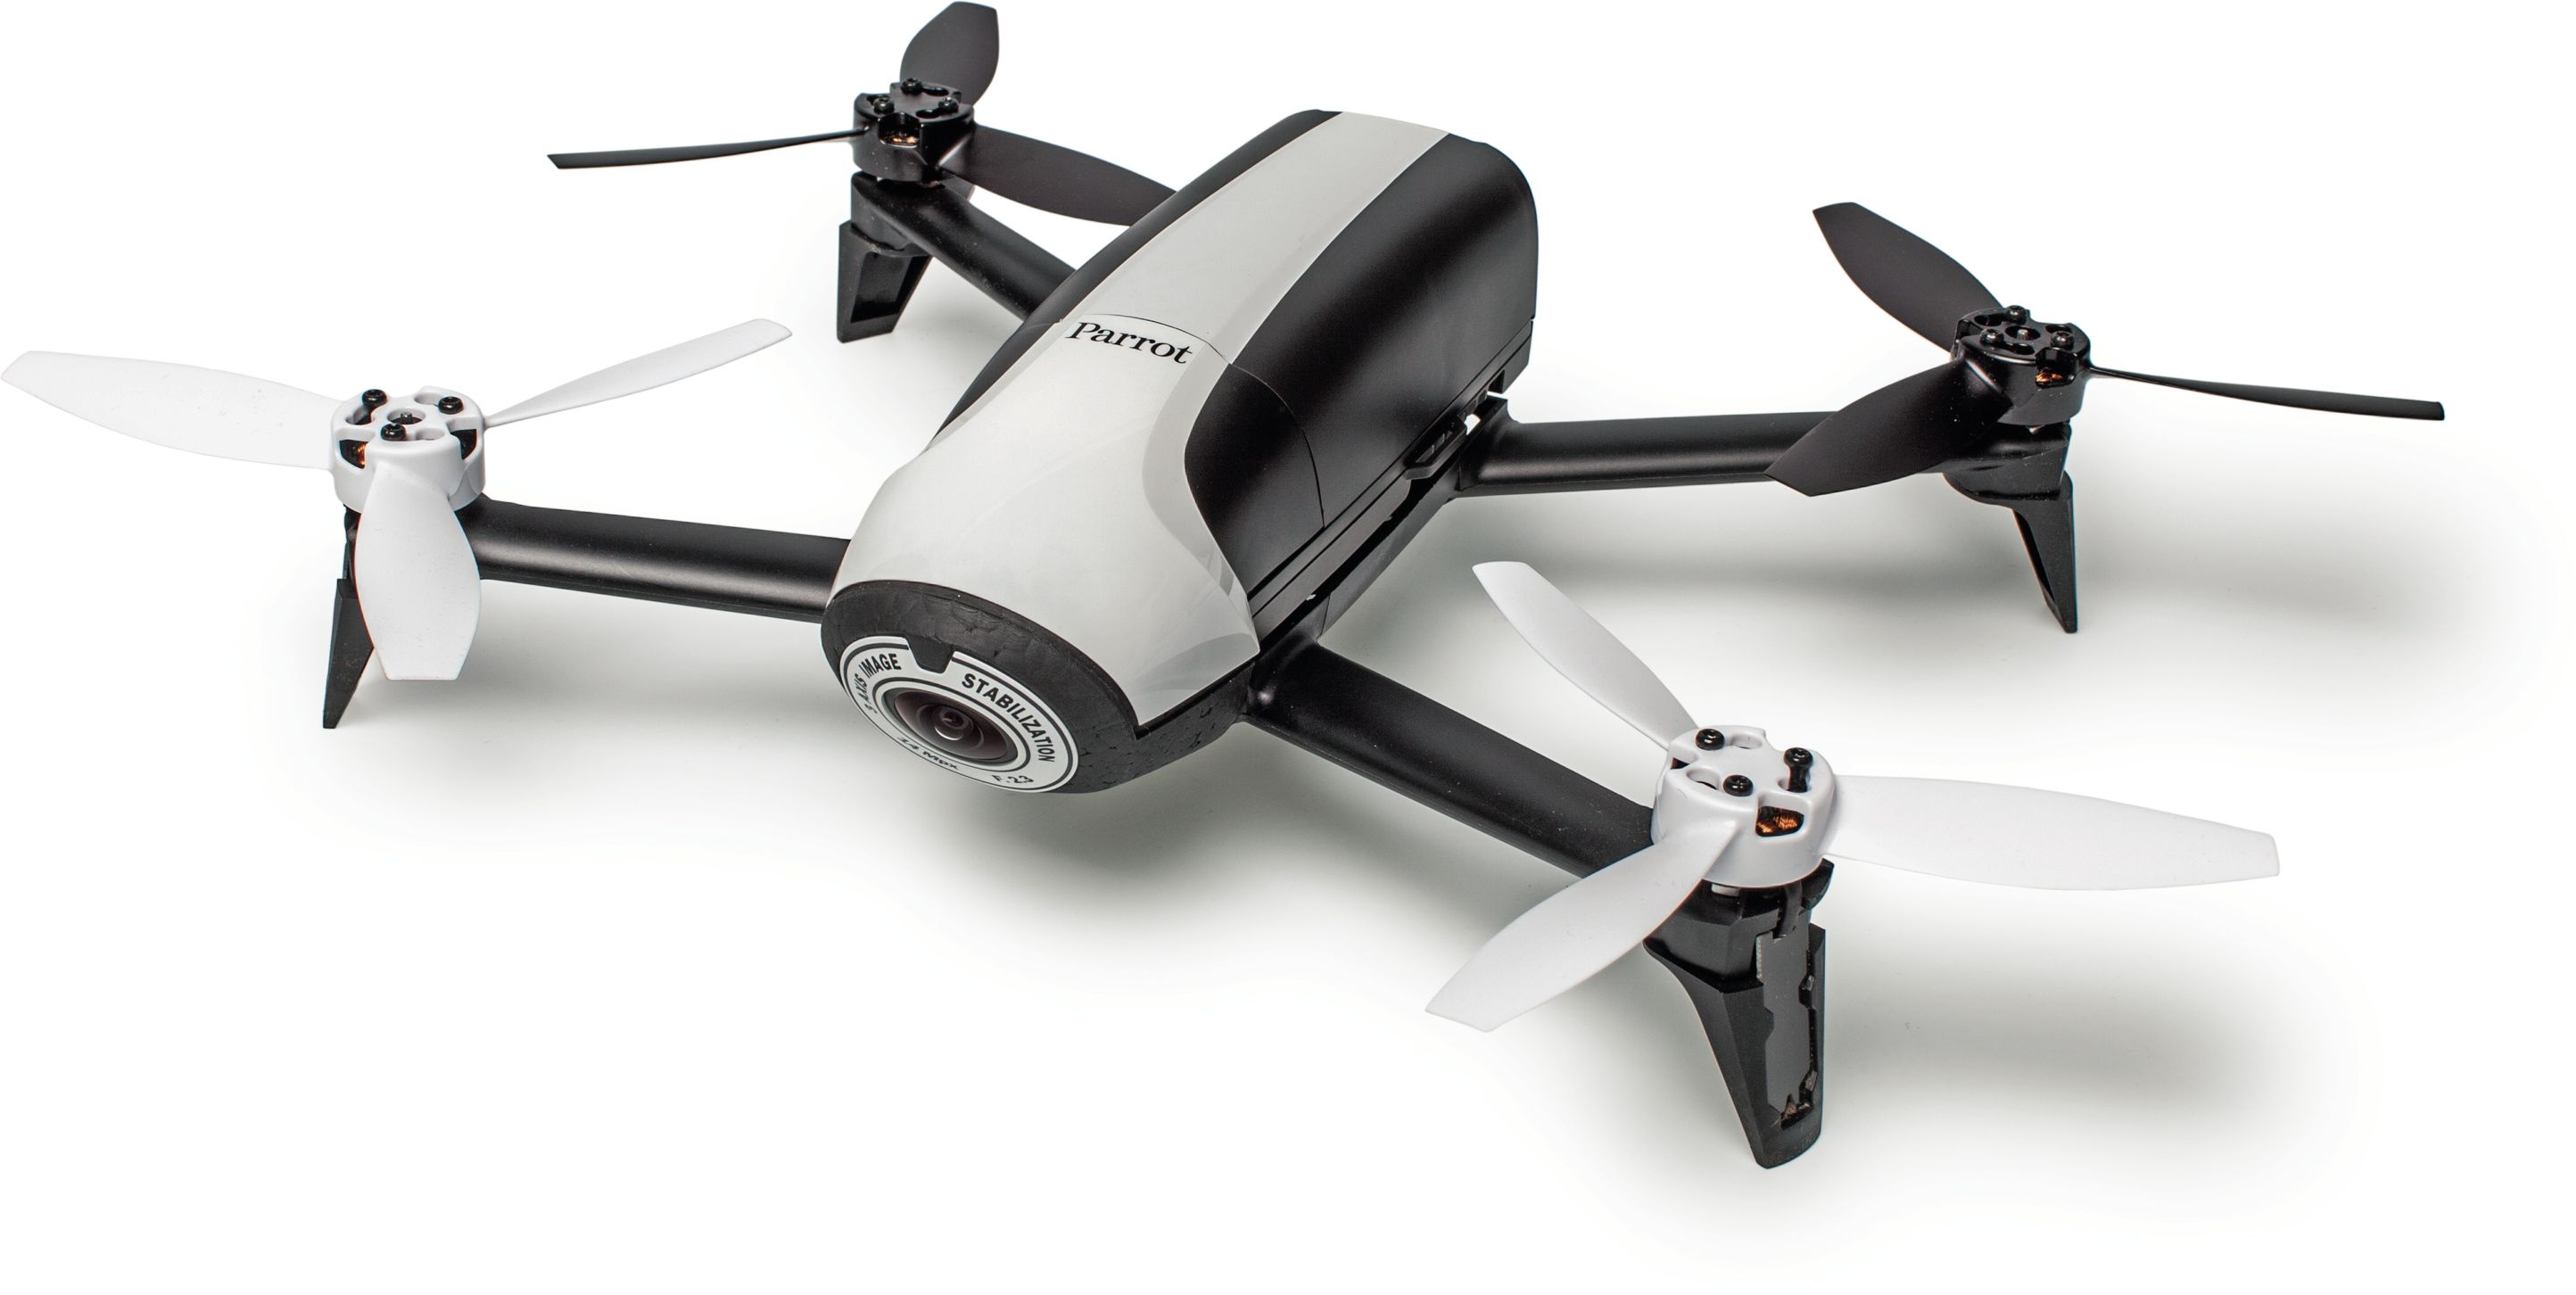
\includegraphics[scale=0.05]{figuras/new_bebop2_branco2} 
%			\caption{Parrot Bebop 2.0 Source: \cite{SAS}}
%		\end{center}
%	\end{figure} & \begin{figure} 
%	\begin{center}
%		
\includegraphics[scale=0.05]{figuras/kinetic.png} 
%		\caption{Parrot Bebop 2.0 Source: }	
%	\end{center}
%\end{figure} &
%\begin{figure} 
%	\begin{center}
%		\includegraphics[scale=0.05]{figuras/90.logo.jpg} 
%		\caption{Parrot Bebop 2.0 Source:}	
%	\end{center}
%\end{figure}
%\end{tabular}

\begin {figure}
\begin{minipage}{0.5\textwidth}
	\centering
	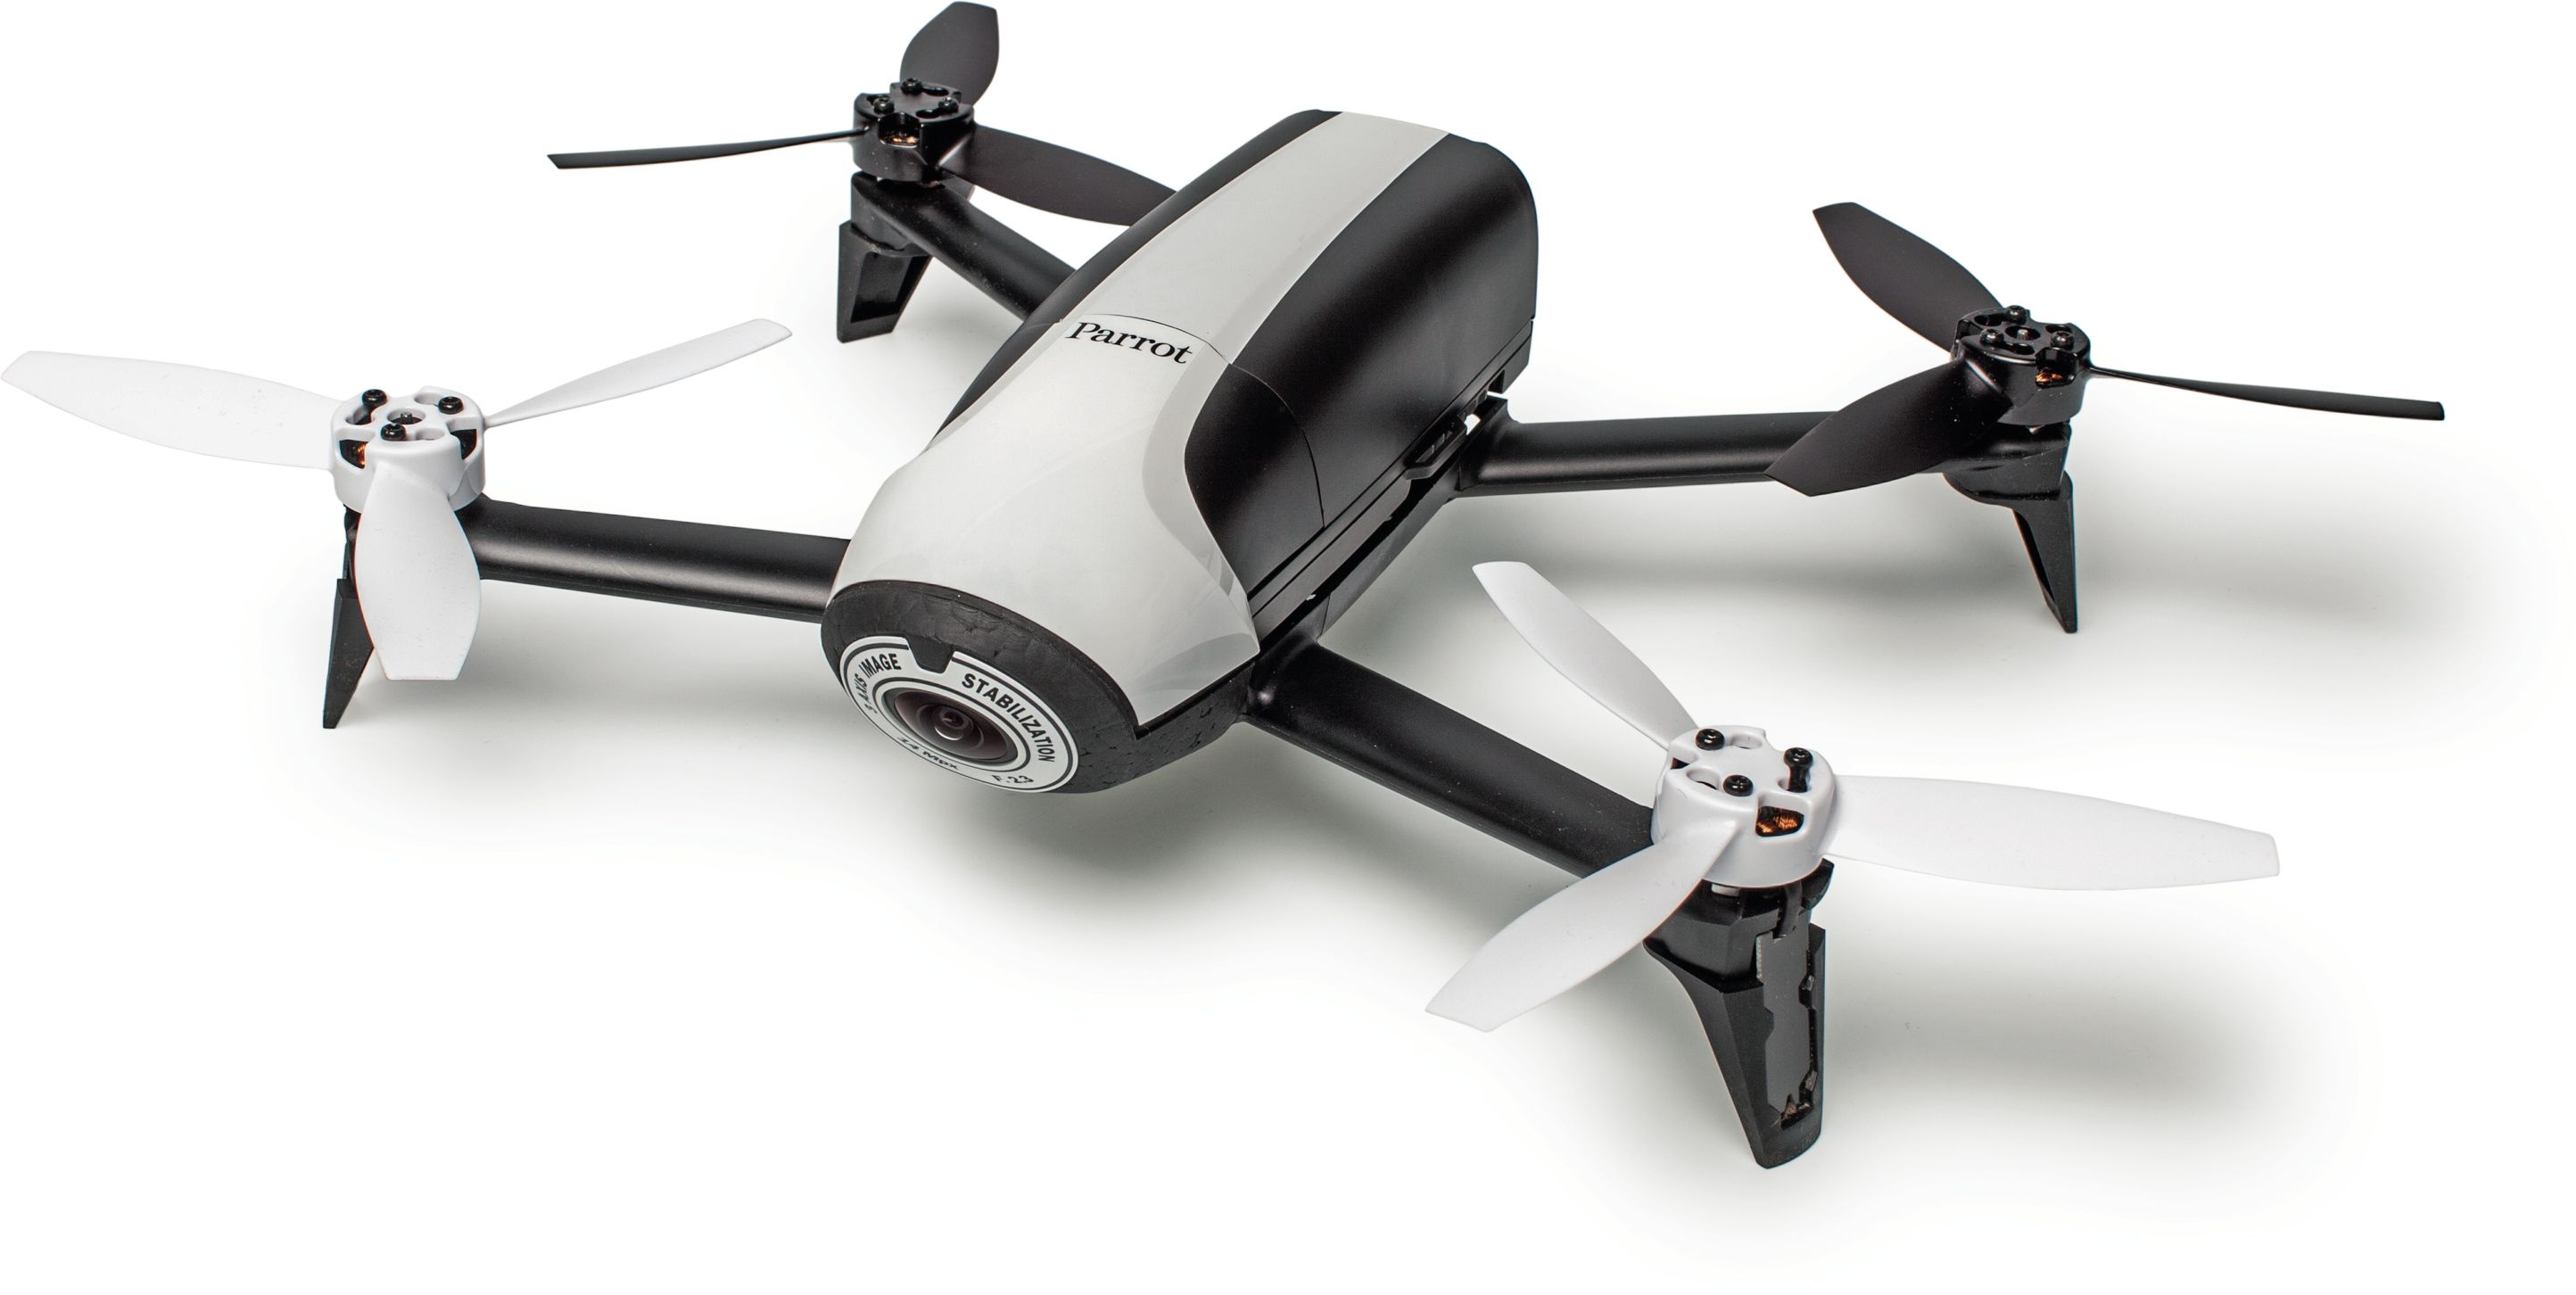
\includegraphics[width=3.5 cm,height=2.4 cm]{figuras/new_bebop2_branco2}
	\caption{Source: \cite{SAS}}
\end{minipage}
\begin{minipage}{0.5\textwidth}
	\centering
	
\includegraphics[width=3.5 cm,height=2.5 cm]{figuras/kinetic.png}
	\caption{Source: Ros.org }
\end{minipage}%
\begin{minipage}{0.5\textwidth}
	\centering
	
\includegraphics[width=3.5 cm,height=2.5 cm]{figuras/vicon}
	\caption{Source: Vicon Motion Systems, Ltd }
\end{minipage}
\end{figure}
\end{frame}

%%%%%%%%%%%%%%%%%%%%%%%%%%%%%%%% FRAME %%%%%%%%%%%%%%%%%%%%%%%%%%%%%%%%

\begin{frame}{Experimental Setup}{Communication\autocite{JRSB2019}}
\begin{figure}[!htb]
	% \includegraphics[trim={5cm 0 0 0},clip]{example-image-a}
	% 	 trim={<left> <lower> <right> <upper>}
	\centering \vspace{-0.4cm}
	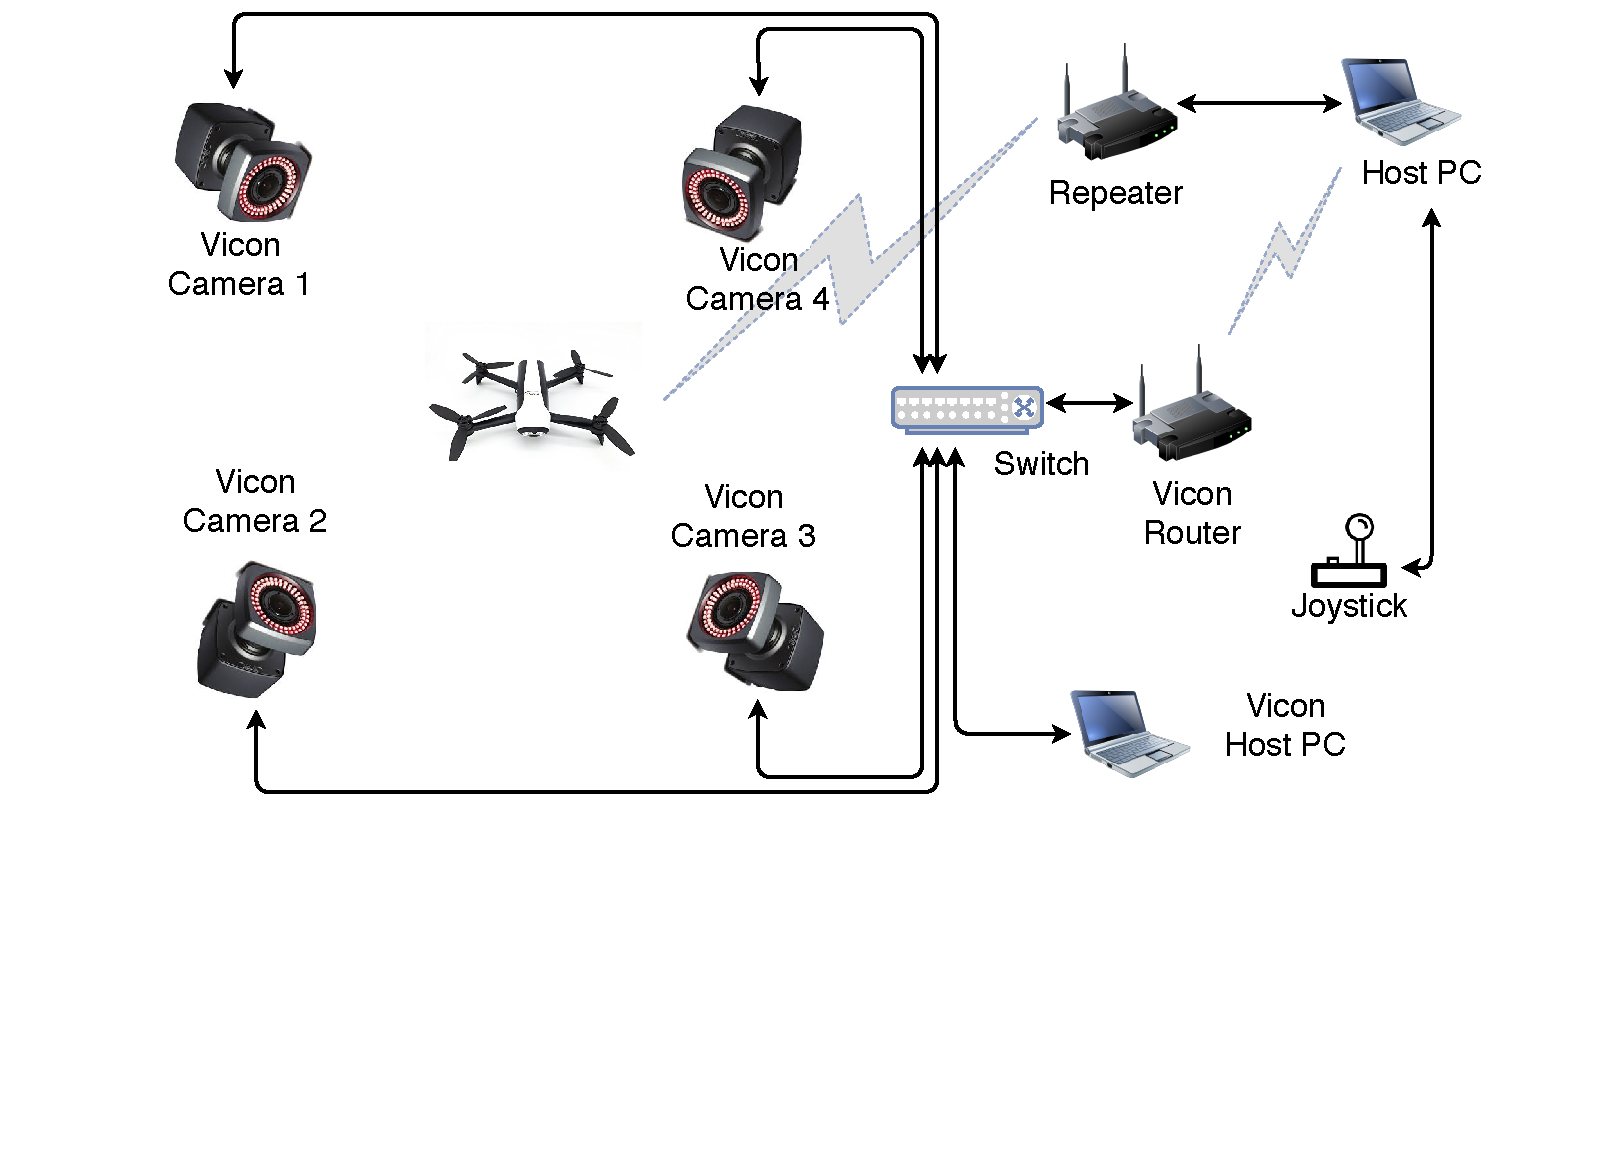
\includegraphics[scale=0.45,trim={28mm 55mm 0 0mm},clip]{figuras/Diagram_ViconDroneDev.pdf}
%	\caption{Source: \citeauthor{JRSB2019} \autocite{JRSB2019}}
	\label{fig:cont_sys}
\end{figure}

\end{frame}

%%%%%%%%%%%%%%%%%%%%%%%%%%%%%%%% FRAME %%%%%%%%%%%%%%%%%%%%%%%%%%%%%%%%

\begin{frame}{Experimental Setup}{Nodes}
\begin{figure}[!htb]
	\centering
	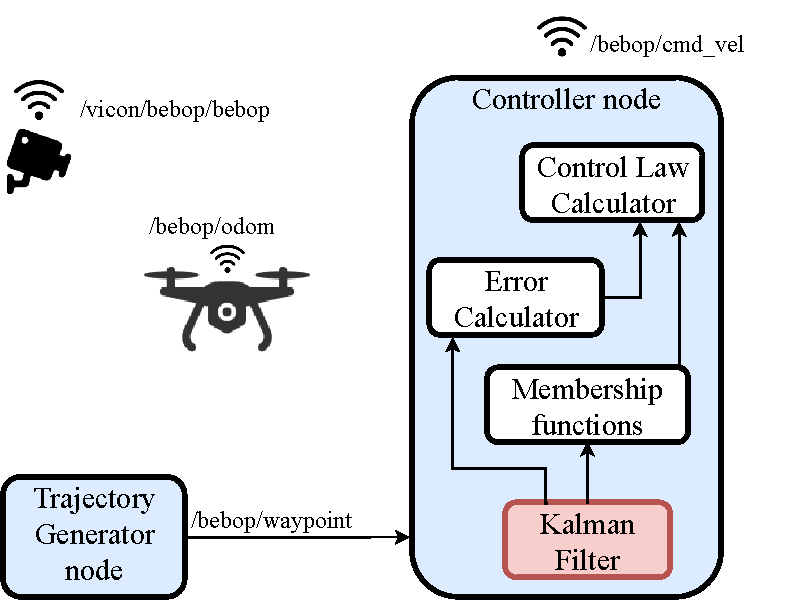
\includegraphics[scale=0.6]{figuras/control_scheme-Page-4.pdf}
	\caption{Source: Author}
	\label{fig:control_scheme}
\end{figure}
\end{frame}

%%%%%%%%%%%%%%%%%%%%%%%%%%%%%%%% FRAME %%%%%%%%%%%%%%%%%%%%%%%%%%%%%%%%

\begin{frame}{Trajectory Generation}{Circle and Lemniscate}
	
	\begin{equation} \label{eq:circle_constant}
	q_d(t) = 
	\begin{bmatrix}
	x_d(t)\\
	y_d(t)\\
	z_d(t)\\
	\psi_d(t)
	\end{bmatrix} = \begin{bmatrix}
	a\cos{\omega t}\\
	a\sin{\omega t}\\
	0\\
	0
	\end{bmatrix}
	\end{equation}
%	where $a$ is the radius and $\omega=\frac{v}{a}$ is the angular velocity. 
%	The variation keeps the front of the drone turned to the center of the circle and is represented in \eqref{eq:circle_center}. We will refer to this trajectory as circle surveillance from now on.
% 	\begin{equation} \label{eq:circle_center}
% 	q_d(t) = 
% 	\begin{bmatrix}
% 	x_d(t)\\
% 	y_d(t)\\
% 	z_d(t)\\
% 	\psi_d(t)
% 	\end{bmatrix} = \begin{bmatrix}
% 	a\cos{\omega t}\\
% 	a\sin{\omega t}\\
% 	0\\
% 	\omega t + \pi
% 	\end{bmatrix}
% 	\end{equation}
%	The last trajectory is an eight-shaped curve, known as the Lemniscate of Gerono. Its equation is given by 
	\begin{equation} \label{eq:lemniscate}
	q_d(t) = 
	\begin{bmatrix}
	x_d(t)\\
	y_d(t)\\
	z_d(t)\\
	\psi_d(t)
	\end{bmatrix} = \begin{bmatrix}
	a\sin{\omega t}\\
	\frac{a}{2}\sin{2\omega t}\\
	0\\
	0
	\end{bmatrix}
	\end{equation}
	\end{frame}

%%%%%%%%%%%%%%%%%%%%%%%%%%%%%%%% FRAME %%%%%%%%%%%%%%%%%%%%%%%%%%%%%%%%
\begin{frame}{State Measurement and estimation}
Only position is available for measurement, so we use a Kalman Filter to estimate velocity.

\vspace{1cm}
Process Model:
\begin{equation} \label{eq:sys_KF}
\zeta(k+1)=\Phi \zeta(k) = \begin{bmatrix}
I & 0 \\
\delta tI & I
\end{bmatrix} \zeta(k)
\end{equation} %where $\zeta$ is the state vector defined in \ref{sec:stSpaceModel}, $\Phi$ is the state transition matrix and $\delta t$ is the time interval it takes to get an update on the position measurement. The observation model is given by 
Measurement Model:
\begin{equation}
m(k)=H \zeta(k) =  \begin{bmatrix}
0 & I
\end{bmatrix}\zeta(k).
\end{equation}
\end{frame}
%%%%%%%%%%%%%%%%%%%%%%%%%%%%%%%% FRAME %%%%%%%%%%%%%%%%%%%%%%%%%%%%%%%%


%%%%%%%%%%%%%%%%%%%%%%%%%%%%%%%% FRAME %%%%%%%%%%%%%%%%%%%%%%%%%%%%%%%%
